\clearpage
\section*{Supplement}
\renewcommand{\thefigure}{S\arabic{figure}}
\setcounter{figure}{0}
\renewcommand{\thetable}{S\arabic{table}}
\setcounter{table}{0}

\newcommand{\cell}[3]{\begin{minipage}[t]{#1}\centering\IfFileExists{#2}{\includegraphics[width=\linewidth]{#2}}{\pendingbox{#3}}\end{minipage}}

\begin{figure}[tbp]
\centering
\cell{0.42\linewidth}{../../results/viz/paper_w3/sw_n4000_dens_k1_kd1_sst15_s1_T8_V0_architecture.png}{architecture}\\[0.8em]
\cell{0.56\linewidth}{../../results/laminar_e2/sw_n4000_dens_k1_kd1_sst15_s1_T8_motif.png}{LFP and SL map}\hfill
\cell{0.42\linewidth}{../../results/viz/paper_w4/sw_n4000_dens_k1_kd1_sst15_s1_T8_csd.png}{CSD}
\caption{Reference column \texttt{e2\_3unit\_n4000\_dens\_k1\_kd1\_sst15}, seed 1, 8 s, exploratory. Top: architecture
as built. Bottom left: model and observed relative-power maps and band profiles. Bottom right: current-based CSD
on alpha troughs. Tables~S1--S4 give the modules, edges per rule, run record and parameters with sources.}
\label{fig:s-reference}
\end{figure}

{\sloppy% Generated by scripts/details_md_to_tex.py from sw_n4000_dens_k1_kd1_sst15_s1_T8_details.md; do not edit by hand.

\begin{table}[p]
\centering\scriptsize
\caption{sw\_n4000\_dens\_k1\_kd1\_sst15\_s1\_T8: Modules.}
\begin{tabular}{lllllll}
\toprule
\textbf{module} & \textbf{depth rel. L4} & \textbf{rho} & \textbf{N\_E} & \textbf{N\_PV} & \textbf{N\_SOM} & \textbf{N} \\
\midrule
S & $-$0.4 & 0.25 & 5,785 & 868 & 217 & 6,870 \\
M & +0.0 & 1 & 3,668 & 344 & 344 & 4,356 \\
D & +0.3 & 2 & 2,547 & 159 & 319 & 3,025 \\
\bottomrule
\end{tabular}
\end{table}

\begin{table}[p]
\centering\scriptsize
\caption{sw\_n4000\_dens\_k1\_kd1\_sst15\_s1\_T8: Edges per rule.}
\begin{tabular}{lllllll}
\toprule
\textbf{rule} & \textbf{pre to post} & \textbf{module or pair} & \textbf{Q (nS)} & \textbf{weight (nS)} & \textbf{mechanism} & \textbf{edges} \\
\midrule
e\_e\_S & E to E & S & 2 & 2 & ampa & 4,684,637 \\
e\_pv\_S & E to PV & S & 3 & 3 & ampa & 705,032 \\
e\_sst\_S & E to SOM & S & 3 & 3 & ampa & 175,640 \\
pv\_e\_S & PV to E & S & 5 & 5 & gaba & 703,143 \\
pv\_pv\_S & PV to PV & S & 5 & 5 & gaba & 105,504 \\
sst\_e\_S & SOM to E & S & 5 & 2.667 & gaba\_sst (15 ms) & 176,231 \\
sst\_pv\_S & SOM to PV & S & 5 & 5 & gaba & 26,316 \\
e\_e\_M & E to E & M & 2 & 2 & ampa & 1,882,762 \\
e\_pv\_M & E to PV & M & 3 & 3 & ampa & 176,635 \\
e\_sst\_M & E to SOM & M & 3 & 3 & ampa & 177,001 \\
pv\_e\_M & PV to E & M & 5 & 5 & gaba & 176,551 \\
pv\_pv\_M & PV to PV & M & 5 & 5 & gaba & 16,577 \\
sst\_e\_M & SOM to E & M & 5 & 2.667 & gaba\_sst (15 ms) & 175,993 \\
sst\_pv\_M & SOM to PV & M & 5 & 5 & gaba & 16,697 \\
e\_e\_D & E to E & D & 2 & 2 & ampa & 907,526 \\
e\_pv\_D & E to PV & D & 3 & 3 & ampa & 56,442 \\
e\_sst\_D & E to SOM & D & 3 & 3 & ampa & 113,463 \\
pv\_e\_D & PV to E & D & 5 & 5 & gaba & 56,463 \\
pv\_pv\_D & PV to PV & D & 5 & 5 & gaba & 3,581 \\
sst\_e\_D & SOM to E & D & 5 & 2.667 & gaba\_sst (15 ms) & 113,760 \\
sst\_pv\_D & SOM to PV & D & 5 & 5 & gaba & 6,958 \\
x\_S\_M\_e\_e & E to E & S$\to$M & 2 & 2 & ampa & 294,237 \\
x\_S\_M\_e\_pv & E to PV & S$\to$M & 3 & 3 & ampa & 27,958 \\
x\_S\_M\_e\_som & E to SOM & S$\to$M & 3 & 3 & ampa & 27,672 \\
x\_M\_S\_e\_e & E to E & M$\to$S & 2 & 2 & ampa & 925,008 \\
x\_M\_S\_e\_pv & E to PV & M$\to$S & 3 & 3 & ampa & 138,762 \\
x\_M\_S\_e\_som & E to SOM & M$\to$S & 3 & 3 & ampa & 34,793 \\
x\_M\_D\_e\_e & E to E & M$\to$D & 2 & 2 & ampa & 408,273 \\
x\_M\_D\_e\_pv & E to PV & M$\to$D & 3 & 3 & ampa & 25,433 \\
x\_M\_D\_e\_som & E to SOM & M$\to$D & 3 & 3 & ampa & 50,841 \\
x\_D\_M\_e\_e & E to E & D$\to$M & 2 & 2 & ampa & 292,676 \\
x\_D\_M\_e\_pv & E to PV & D$\to$M & 3 & 3 & ampa & 27,622 \\
x\_D\_M\_e\_som & E to SOM & D$\to$M & 3 & 3 & ampa & 27,430 \\
\bottomrule
\end{tabular}
\end{table}

\begin{table}[p]
\centering\scriptsize
\caption{sw\_n4000\_dens\_k1\_kd1\_sst15\_s1\_T8: Run.}
\begin{tabular}{ll}
\toprule
\textbf{key} & \textbf{value} \\
\midrule
layout & e2\_3unit\_n4000\_dens\_k1\_kd1\_sst15 \\
experiment & E2 stack, first pass (unsealed; owner rulings 2026-11-09) \\
seed & 1 \\
T\_s & 8 \\
dt\_ms & 0.1 \\
jaxfne\_version & 0.5.9 \\
jaxfne\_source sha & not recorded \\
jax\_devices & ['cpu:0'] \\
git\_sha (run) & 5992eb736979e731aba788892346761926393cfc \\
git\_dirty & not recorded in run JSON \\
wall\_s & 2367.11 \\
\bottomrule
\end{tabular}
\end{table}

\clearpage
{\scriptsize
\begin{longtable}{lp{3.6cm}p{2.6cm}lp{6.2cm}}
\caption{sw\_n4000\_dens\_k1\_kd1\_sst15\_s1\_T8: Parameters.}\\
\toprule
\textbf{group} & \textbf{parameter} & \textbf{value} & \textbf{unit} & \textbf{source} \\
\midrule
\endfirsthead
\toprule
\textbf{group} & \textbf{parameter} & \textbf{value} & \textbf{unit} & \textbf{source} \\
\midrule
\endhead
\bottomrule
\endlastfoot
neuron & E VT\_mV & -50 & mV & PORT\_SPEC (Tahvili, Vinck, di Volo) \\
neuron & PV VT\_mV & -50 & mV & PORT\_SPEC (Tahvili, Vinck, di Volo) \\
neuron & SOM VT\_mV & -50 & mV & PORT\_SPEC (Tahvili, Vinck, di Volo) \\
neuron & E Delta\_mV & 2 & mV & PORT\_SPEC (Tahvili, Vinck, di Volo) \\
neuron & PV Delta\_mV & 0.5 & mV & PORT\_SPEC (Tahvili, Vinck, di Volo) \\
neuron & SOM Delta\_mV & 2 & mV & PORT\_SPEC (Tahvili, Vinck, di Volo) \\
neuron & E Tref\_ms & 5 & ms & PORT\_SPEC (Tahvili, Vinck, di Volo) \\
neuron & PV Tref\_ms & 5 & ms & PORT\_SPEC (Tahvili, Vinck, di Volo) \\
neuron & SOM Tref\_ms & 5 & ms & PORT\_SPEC (Tahvili, Vinck, di Volo) \\
neuron & E tauw\_ms & 500 & ms & PORT\_SPEC (Tahvili, Vinck, di Volo) \\
neuron & PV tauw\_ms & 500 & ms & PORT\_SPEC (Tahvili, Vinck, di Volo) \\
neuron & SOM tauw\_ms & 500 & ms & PORT\_SPEC (Tahvili, Vinck, di Volo) \\
neuron & E a\_nS & 4 & nS & PORT\_SPEC (Tahvili, Vinck, di Volo) \\
neuron & PV a\_nS & 0 & nS & PORT\_SPEC (Tahvili, Vinck, di Volo) \\
neuron & SOM a\_nS & 4 & nS & PORT\_SPEC (Tahvili, Vinck, di Volo) \\
neuron & E b\_pA & 50 & pA & PORT\_SPEC (Tahvili, Vinck, di Volo) \\
neuron & PV b\_pA & 0 & pA & PORT\_SPEC (Tahvili, Vinck, di Volo) \\
neuron & SOM b\_pA & 80 & pA & PORT\_SPEC (Tahvili, Vinck, di Volo) \\
neuron & E C\_pF & 200 & pF & PORT\_SPEC (Tahvili, Vinck, di Volo) \\
neuron & PV C\_pF & 200 & pF & PORT\_SPEC (Tahvili, Vinck, di Volo) \\
neuron & SOM C\_pF & 200 & pF & PORT\_SPEC (Tahvili, Vinck, di Volo) \\
neuron & E gL\_nS & 10 & nS & PORT\_SPEC (Tahvili, Vinck, di Volo) \\
neuron & PV gL\_nS & 10 & nS & PORT\_SPEC (Tahvili, Vinck, di Volo) \\
neuron & SOM gL\_nS & 10 & nS & PORT\_SPEC (Tahvili, Vinck, di Volo) \\
neuron & E EL\_mV & -65 & mV & PORT\_SPEC (Tahvili, Vinck, di Volo) \\
neuron & PV EL\_mV & -65 & mV & PORT\_SPEC (Tahvili, Vinck, di Volo) \\
neuron & SOM EL\_mV & -55 & mV & PORT\_SPEC (Tahvili, Vinck, di Volo) \\
neuron & E Vreset\_mV & -65 & mV & PORT\_SPEC (Tahvili, Vinck, di Volo) \\
neuron & PV Vreset\_mV & -65 & mV & PORT\_SPEC (Tahvili, Vinck, di Volo) \\
neuron & SOM Vreset\_mV & -65 & mV & PORT\_SPEC (Tahvili, Vinck, di Volo) \\
neuron & spike registered at & V $\geq$ VT + 5 Delta & mV & PORT\_SPEC (Tahvili, Vinck, di Volo) \\
synapse & tau\_delay & 2 & ms & PORT\_SPEC (Tahvili, Vinck, di Volo) \\
synapse & tau\_E (AMPA) & 2 & ms & PORT\_SPEC (Tahvili, Vinck, di Volo) \\
synapse & tau\_I (GABA) & 8 & ms & PORT\_SPEC (Tahvili, Vinck, di Volo) \\
synapse & E\_rev E (AMPA) & 0 & mV & PORT\_SPEC (Tahvili, Vinck, di Volo) \\
synapse & E\_rev I (GABA) & -80 & mV & PORT\_SPEC (Tahvili, Vinck, di Volo) \\
synapse & Q E$\to$E & 2 & nS & PORT\_SPEC (Tahvili, Vinck, di Volo) \\
synapse & Q E$\to$PV, E$\to$SOM & 3 & nS & PORT\_SPEC (Tahvili, Vinck, di Volo) \\
synapse & Q PV$\to$E, PV$\to$PV, SOM$\to$E, SOM$\to$PV & 5 & nS & PORT\_SPEC (Tahvili, Vinck, di Volo) \\
synapse & Q PV$\to$SOM, SOM$\to$SOM & 0 & nS & PORT\_SPEC (Tahvili, Vinck, di Volo) (absent in the reference model) \\
drive & Q external $\to$ E, PV & 2.5 & nS & PORT\_SPEC (Tahvili, Vinck, di Volo) \\
drive & external sources per E and PV cell & 560 & count & PORT\_SPEC (Tahvili, Vinck, di Volo) (round(p NE), p 0.07; per-cell sources are the port's assumption) \\
drive & external rate per source & 4 & Hz & PORT\_SPEC (Tahvili, Vinck, di Volo) \\
drive & external drive to SOM & none &  & PORT\_SPEC (Tahvili, Vinck, di Volo) \\
network & dt & 0.1 & ms & PORT\_SPEC (Tahvili, Vinck, di Volo) (Brian2 Euler dt; caminos\_e0 DT\_MS) \\
network & N\_E, N\_PV, N\_SOM (reference) & 8000, 750, 750 & count & PORT\_SPEC (Tahvili, Vinck, di Volo) \\
network & within-module p (CAMINOS) & 0.07 &  & PORT\_SPEC (Tahvili, Vinck, di Volo) \\
network & K\_E = N\_E p (E inputs per cell) & 560 & count & PORT\_SPEC (Tahvili, Vinck, di Volo) (caminos\_stack.K\_E) \\
network & K\_INTER (inter-module E inputs per cell per neighbour) & 80 & count & agent choice (caminos\_stack.K\_INTER; the code comment cites owner ruling 2026-11-09 for p 0.01 of 8000) \\
network & k (inter-module in-degree scale) & 1 &  & agent choice (set) \\
network & inter-module in-degree per target E cell & 80 from each neighbour; end module 160 from its one neighbour & count & caminos\_stack.build\_config; K\_INTER agent choice \\
network & inter-module p & null: K\_INTER based &  & run JSON p\_inter; caminos\_stack.build\_config \\
network & within-module p (S) & 0.139997 &  & derived: K\_E/N\_E x (density/mean density)\textasciicircum{}kd (caminos\_stack.local\_p); kd agent choice \\
network & within-module p (M) & 0.14 &  & derived: K\_E/N\_E x (density/mean density)\textasciicircum{}kd (caminos\_stack.local\_p); kd agent choice \\
network & within-module p (D) & 0.140008 &  & derived: K\_E/N\_E x (density/mean density)\textasciicircum{}kd (caminos\_stack.local\_p); kd agent choice \\
synapse & SOM$\to$E tau (S) & 15 & ms & agent choice (sst modifier) \\
synapse & SOM$\to$E weight (S) & 2.66667 & nS & derived: Q\_INH x TAU\_I/tau (caminos\_stack.build\_config); tau agent choice \\
synapse & SOM$\to$E tau (M) & 15 & ms & agent choice (sst modifier) \\
synapse & SOM$\to$E weight (M) & 2.66667 & nS & derived: Q\_INH x TAU\_I/tau (caminos\_stack.build\_config); tau agent choice \\
synapse & SOM$\to$E tau (D) & 15 & ms & agent choice (sst modifier) \\
synapse & SOM$\to$E weight (D) & 2.66667 & nS & derived: Q\_INH x TAU\_I/tau (caminos\_stack.build\_config); tau agent choice \\
module & rho = N\_SOM/N\_PV (S) & 0.25 &  & owner ruling 2026-11-09 (caminos\_stack.RHO comment); rho 1 = PORT\_SPEC 750/750 \\
module & depth rel L4 (S) & -0.4 &  & agent choice (caminos\_stack.layout) \\
module & rho = N\_SOM/N\_PV (M) & 1 &  & owner ruling 2026-11-09 (caminos\_stack.RHO comment); rho 1 = PORT\_SPEC 750/750 \\
module & depth rel L4 (M) & 0 &  & agent choice (caminos\_stack.layout) \\
module & rho = N\_SOM/N\_PV (D) & 2 &  & owner ruling 2026-11-09 (caminos\_stack.RHO comment); rho 1 = PORT\_SPEC 750/750 \\
module & depth rel L4 (D) & 0.3 &  & agent choice (caminos\_stack.layout) \\
module & MODULE\_BINS (S) & -0.6 to -0.2 (9 bins) &  & agent choice (caminos\_stack.MODULE\_BINS on lansa\_density\_X.json bins) \\
module & MODULE\_BINS (M) & -0.15 to 0.15 (7 bins) &  & agent choice (caminos\_stack.MODULE\_BINS on lansa\_density\_X.json bins) \\
module & MODULE\_BINS (D) & 0.2 to 0.4 (5 bins) &  & agent choice (caminos\_stack.MODULE\_BINS on lansa\_density\_X.json bins) \\
modifier & n (mean E cells per module) & 4000 & count & agent choice (layout modifier n) \\
modifier & dens (E cells proportional to LANSA density) & on &  & agent choice (layout modifier dens) \\
modifier & kd (local in-degree exponent) & 1 &  & agent choice (layout modifier kd) \\
modifier & sst (SOM$\to$E decay, all modules) & 15 & ms & agent choice (layout modifier sst) \\
analysis & sigma (probe Gaussian, relative depth) & 0.15 &  & agent choice (e2\_motif\_figure.SIGMA) \\
analysis & V\_ref (current proxy) & -65 & mV & agent choice (e2\_motif\_figure.V\_REF\_MV) \\
analysis & discard & 2 & s & PLAN\_LANSA\_E2.md, C6 (2 s discarded) \\
analysis & multitaper half-bandwidth (smoothing) & 2 & Hz & e2\_motif\_figure.SMOOTH\_HZ (as the published analysis) \\
analysis & RWS delay & 6 & ms & Mazzoni et al. 2015 (e2\_motif\_figure.py; plan section 0) \\
analysis & RWS alpha & 1.65 &  & Mazzoni et al. 2015 (e2\_motif\_figure.py; plan section 0) \\
analysis & bands alpha-beta / gamma & 10-30 / 50-150 & Hz & owner ruling 2026-11-09 (PLAN\_LANSA\_E2.md, Owner rulings) \\
analysis & probe contacts & 21 at -0.6 to 0.4 rel. L4 &  & LANSA bin centres (lansa\_density\_X.json axes; e2\_motif\_figure.CHANNELS) \\
\end{longtable}}

\paragraph{Notes to the sw\_n4000\_dens\_k1\_kd1\_sst15\_s1\_T8 tables.}
{\small\begin{itemize}
\item Total N = 14,251.
\item Exploratory, unsealed E2 run (run JSON experiment). The recorded JaxFNE version is 0.5.9; PLAN\_LANSA\_E2.md section 0 and OPEN-37 name 0.5.8 as the project authority.
\item Raster: sampled cells only (200 E, 50 PV and 50 SOM per module, a random sample by run\_e2\_stack.py).
\item Module N is the sum of the recorded cell counts; the run JSON has no N key.
\item Local p and the inter-module edges are as recorded; the inter-module autapse rule is not checked here.
\item Run JSON has no git\_dirty, jaxfne\_source key (written by later runner versions); reported as not recorded.
\item tau\_sst\_e\_ms is a scalar in the run JSON; the current runner writes a per-module dict (caminos\_stack.sst\_taus). Both are read the same way here.
\end{itemize}}
}

\begin{figure}[tbp]
\centering
\IfFileExists{../../results/viz/paper_w6/seed_diff.png}{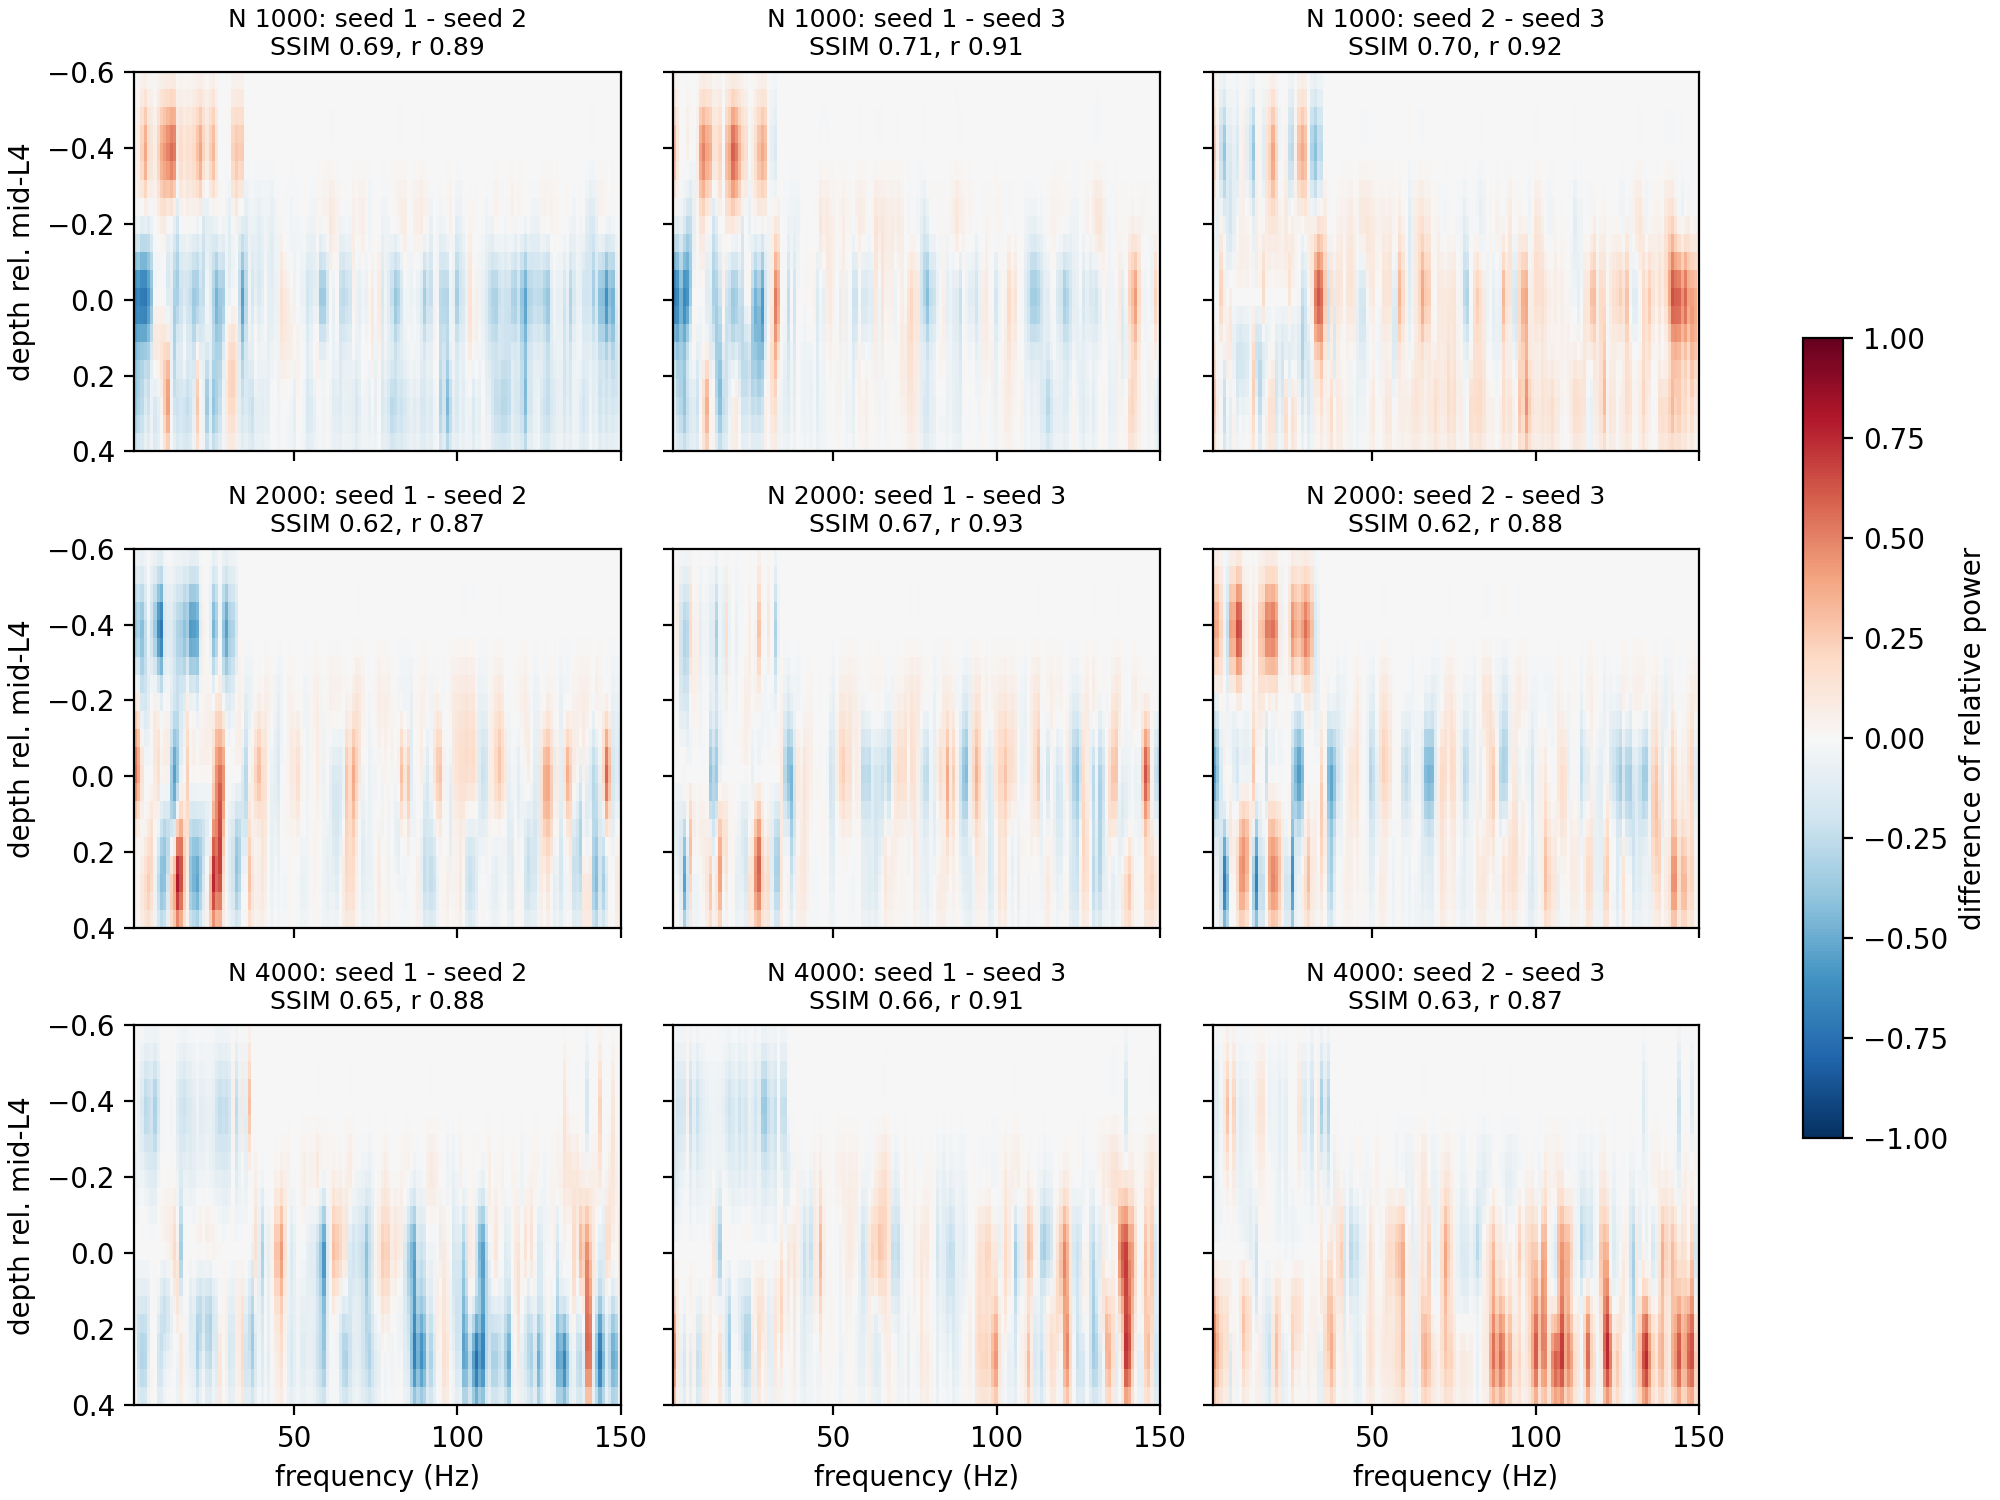
\includegraphics[width=\linewidth]{../../results/viz/paper_w6/seed_diff.png}}{\pendingbox{seed differences}}
\caption{Seed agreement on the finite-size ladder. Seed pairs: SSIM 0.62--0.71, pixel $r$ 0.87--0.93; each seed
against the observed map: SSIM 0.04--0.12, $r$ 0.20--0.43 (\texttt{results/viz/paper\_w6/seed\_diff.json}).}
\label{fig:seeds}
\end{figure}

\begin{figure}[tbp]
\centering
\panel{N1000 s1}{../../results/laminar_e2/lfs_n1000_s1_T8_motif.png}{0.32\linewidth}{missing}\hfill
\panel{N1000 s2}{../../results/laminar_e2/lfs_n1000_s2_T8_motif.png}{0.32\linewidth}{missing}\hfill
\panel{N1000 s3}{../../results/laminar_e2/lfs_n1000_s3_T8_motif.png}{0.32\linewidth}{missing}\\[0.8em]
\panel{N2000 s1}{../../results/laminar_e2/lfs_n2000_s1_T8_motif.png}{0.32\linewidth}{missing}\hfill
\panel{N2000 s2}{../../results/laminar_e2/lfs_n2000_s2_T8_motif.png}{0.32\linewidth}{missing}\hfill
\panel{N2000 s3}{../../results/laminar_e2/lfs_n2000_s3_T8_motif.png}{0.32\linewidth}{missing}\\[0.8em]
\panel{N4000 s1}{../../results/laminar_e2/sw_n4000_dens_k1_kd1_sst15_s1_T8_motif.png}{0.32\linewidth}{missing}\hfill
\panel{N4000 s2}{../../results/laminar_e2/lfs_n4000_s2_T8_motif.png}{0.32\linewidth}{missing}\hfill
\panel{N4000 s3}{../../results/laminar_e2/lfs_n4000_s3_T8_motif.png}{0.32\linewidth}{missing}
\caption{Finite-size ladder motif maps, one per $N$ and seed; scores in Table~\ref{tab:ladder}. Ladder rule (\texttt{results/laminar\_e2/lfs\_rule.json}): seed-mean
$r_\text{proto}$ 0.334, 0.387, 0.328 for $N$ = 1000, 2000, 4000; both smaller $N$ are within 2 SD of $N = 4000$ in
$r_\text{proto}$ but fail the 3 Hz peak test on the S unit (seed-mean S peak 8, 31, 43 Hz), so the T1 size is
$N = 4000$.}
\label{fig:s-ladder}
\end{figure}

\begin{table}[tbp]
\centering
\small
\begin{tabular}{lp{0.42\linewidth}ll}
\toprule
Test & Manipulation & Seal & Status \\
\midrule
T2 & every GABA weight $\times g$, $g \in \{0.25,\ldots,4\}$ & \path{SEAL_T2_T3.md} & sealed, not run \\
T3 & every unit's $N_\text{SOM}/N_\text{PV} \times s$, $s \in \{0.25,\ldots,4\}$ & \path{SEAL_T2_T3.md} & sealed, not run \\
T4 & PV or SOM silencing and $+50$ pA stimulation per unit & \path{SEAL_T4.md} & sealed, not run \\
T5 & VIP population & none & deferred (AdEx has no VIP) \\
\bottomrule
\end{tabular}
\caption{Sealed or planned tests not run for this report (seals in \texttt{docs/laminar\_motif/}).}
\label{tab:notrun}
\end{table}
